\documentclass[conference]{IEEEtran}

\usepackage[utf8x]{inputenc}

\usepackage{dcolumn}
\usepackage{graphicx}
\usepackage{epsfig}
\usepackage{amssymb}
\usepackage{amsmath}
\usepackage{amsfonts}
\usepackage{subcaption}
\usepackage{multirow}
\usepackage{color}
\usepackage{array}
\usepackage{listings}
\lstset{language=C}

\usepackage{times}

\begin{document}

\title{Software-defined network support for transport resilience}

%\author{
%\alignauthor Jo\~{a}o Taveira Ara\'{u}jo\\
%        \email{j.araujo@ucl.ac.uk}
%\alignauthor Raul Landa \\
%        \email{r.landa@ucl.ac.uk}
%\alignauthor Kensuke Fukuda \\
%        \email{kensuke@nii.ac.jp}
%\alignauthor George Pavlou \\
%        \email{g.pavlou@ucl.ac.uk}
%\end{tabular}\newline\begin{tabular}{cc}
%    \affaddr{University College London} & \affaddr{University College London}\\
%    \affaddr{London, UK} & \affaddr{London, UK}\\
%}


% author names and affiliations
% use a multiple column layout for up to three different
% affiliations
\author{\IEEEauthorblockN{Jo\~{a}o Taveira Ara\'{u}jo, Ra\'{u}l Landa, Richard G. Clegg, George Pavlou}
\IEEEauthorblockA{University College London\\
Email: \{j.araujo, r.landa, r.clegg, g.pavlou\}@ucl.ac.uk}}
%\and
%\IEEEauthorblockN{Kensuke Fukuda}
%\IEEEauthorblockA{National Institute of Informatics\\
%kensuke@nii.ac.jp}}

\maketitle

\maketitle
\begin{abstract}
Existing methods for traffic resilience at the network and transport layers typically work in isolation, often resorting to inference in fault detection and recovery respectively.
This both duplicates functionality across layers, eroding efficiency, and leads to protracted recovery cycles, affecting responsiveness.
Such misalignment is particularly at odds with the unprecedented concentration of traffic in data-centers, in which network and hosts are managed in unison.

This paper advocates instead a cross-layer approach to traffic resilience.
The proposed architecture, INFLEX, builds on the abstractions provided by software-defined networking (SDN) to maintain multiple virtual forwarding planes which the network assigns to flows.
In case of path failure, transport protocols pro-actively request to switch plane in a manner which is unilaterally deployable by an edge domain, providing scalable end-to-end forwarding path resilience.


\end{abstract}

\section{Introduction}

% generic "failures are bad"
Despite being broadly designed for robustness, the current Internet architecture remains remarkably vulnerable to failures.
Managing faults effectively poses a significant operational challenge, in part because faults differ widely in both source and nature, potentially occuring at any layer of the stack and along any element along a path.

% neither is transport
\LOREM
\LOREM

% network methods
Given the commercial nature of the Internet, the onus of providing resilience has instead shifted to network operators.
Traditionally this has been achieved by overloading the routing architecture.
The deployment of real time applications with harder constraints on reliability coupled with better failure detection methods embedded in linecards have provided both the motivation and the means for achieving sub-second recovery within IGP networks \cite{}.
Even with reduced recovery times however, the transient effects of routing changes can still disrupt the forwarding path. 
Under such cases diverse proposals such as Fast Re-Route \cite{}, Loop-Free Alternate next hops \cite{} or Packet Re-cycling \cite{} can provide repair paths for use between the detection of a failure and the convergence of the routing process.

Unfortunately, such methods are rarely sufficient.
Firstly, their application is circumscribed to individual domains, and as such cannot provide end-to-end coverage in a federated, best-effort Internet.
Secondly, there are many faults which do not directly pertain to routing, such as middlebox misconfiguration or hardware malfunctions, and as such go undetected.
Finally, reparation often disregards and potentially disrupts the transport layer by causing out-of-order delivery of packets.

% why now. datacenter, SDN
\LOREM
\LOREM
\LOREM

% layout?
\LOREM
\LOREM


%Outside their networks however, operators are reduced to negotiating service level agreements with their own providers who are invariably unable to cater for such specialized demands \cite{}.
%Even if such terms were met, the Internet architecture provides limited visibility beyond one's own domain.
%This opaqueness, in addition to the fact that failures themselves may be distributed in nature \cite{}, severely limits the ability for a customer network to trace remote problems to a single source \cite{}.
%With no means to hold providers accountable for failures, there is little to enforce the terms of a truly end-to-end SLA.
%
%Unfortunately, such intradomain methods 


%Alongside this increased centralization of resources comes a heightened sense of accountability.
%The commercial nature of the agreements between customers and cloud hosting companies such as AWS \cite{} often involve the establishment of service level agreements.
%Even where such agreements are not explicit, such as the base option of tiered services such as Dropbox or Heroku, there is an inherent need to minimize the impact of outages -- non paying customers may be less demanding, but they are also less sensitive to the switching cost incurred in changing service provider.
%
%Unfortunately, the federated, best-effort nature of the Internet seemingly does not lend itself to such high expectations.



%Under such cases, a network operator is currently expected to detect, repair and recover from such faults.
%Detection often requires scale -- the reliability with which a fault can be identified relies on the proportion of traffic affected. 
%In many cases, faults affecting single flows may go undetected by the network.
%Once detected, reparation varies according to the nature and origin of the fault.
%For some cases, such as intradomain routing, this process is often automated and robust.
%For many others however, such as faulty hardware or misconfigured devices, recovery is difficult and error-prone.
%In either case, the amount of time expended in detection and repair can often preclude recovery, since most flows will terminate after successive timeouts.
%

%Fueled largely by economies of scale in both software management and hardware acquisition and maintenance, the emergence of cloud computing and content distribution networks has lead to a profound shift in Internet traffic.
%
%
%Whereas the advent of broadband connections init
%In contrast to the highly distributed nature of peer-to-peer software which 
%
%
%For one, never has so much been distributed by so few to so many.
%% AS dist graph
%% netflix
%
%\LOREM
%
%% Accountability, resilience

%All intervening equipment is subject to failure along a network path, with recovery time depending not only on \emph{what} happened, but also \emph{where}.
%Within their networks, operators are free to instrument and deploy arbitrarily complex tools to meet requirements. 
%This freedom has lead to a proliferation of proposed improvements in resilience for intradomain settings \cite{}.


%The establishment of SLAs for network availability have traditionally been prefered within the telecom industry in particular, and represent one possible approach to ensuring resilience. An alternative approach is offered by the end-to-end principle. 
%Since end hosts possess both inherent knowledge of application needs and fine-grained measurements on end-to-end path characteristics, the transport layer is often identified as a more natural fit for dealing with fault tolerance at an Internet scale.
%Both SCTP \cite{} and MPTCP \cite{} enable transparent fail-over through multihoming.
%In spite of providing significant features, neither is likely to be widely deployed in the near future: the former lacks critical middlebox support, while the latter is still undergoing standardization.
%Furthermore, the requirement for end-host multihoming has also posed a barrier to deployment.
%Finally, all transport approaches to fail-over confine knowledge of faults within an individual flow: each flow must detect failures independently, even when many flows are affected by the same fault.
%


% Transport is not the answer

% Can we do better with SDN?


%A default forwarding plane, corresponding to the label 0, must be defined and cater for all traffic destinations.
%As with existing routing infrastructure, this single default plane will suffice for most traffic.

%Invariably however, path failures will arise which may affect any number of flows.
%Rather than expecting the network to address end-to-end failures, hosts are allowed to proactively request an overlay plane from the network.





\section{Openflow background}
\label{section:inflex:background}

A valuable development in assisting traffic management has been the emergence of \ac{SDN}, which can facilitate vastly improved flexibility for scalable, policy-based network control.
Software defined networks decouple the data plane and control plane, allowing both to evolve independently.
A traditional instantiation of a software defined network for data centres is shown in figure \ref{fig:ofparch}.
Each physical host runs a number of virtual machines, each connected locally through a edge, software-based switch (such as OpenVSwitch \cite{openvswitch}) running on the underlying physical host operating system, which will be denoted as \emph{dom0}.
This switch is in turn connected to further forwarding devices, ensuring access to a wider network.
The forwarding logic of each device can be accessed and configured by a controller through the establishment of a control channel through a common protocol, of which Openflow is the most widely used \cite{McKeown:2008:OEI:1355734.1355746}.
Both software and physical switches are indistinguishable from a controller's perspective: \emph{how} a device implements Openflow is immaterial, so long as a forwarding device conforms to the given \ac{API}.

\begin{figure}
    \centering
    \begin{subfigure}[b]{0.5\linewidth}
    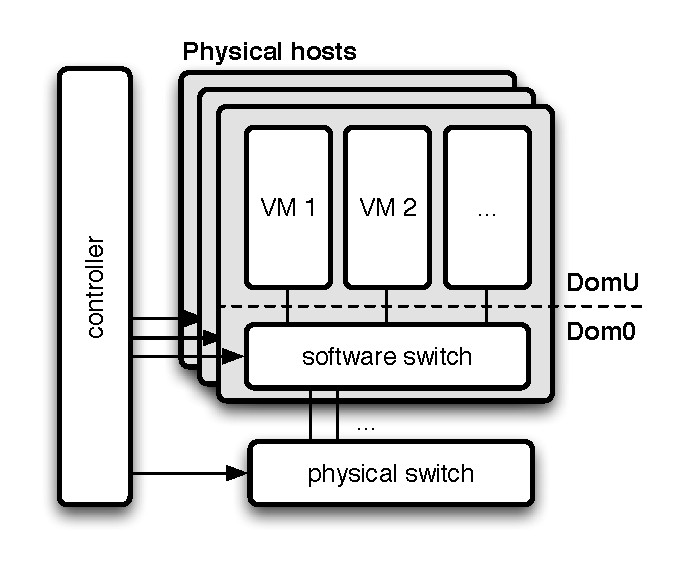
\includegraphics[width=0.9\linewidth]{figures/inflex/ofparch}
    \caption{\label{fig:ofparch}}
    \end{subfigure}%
    \begin{subfigure}[b]{0.5\linewidth}
    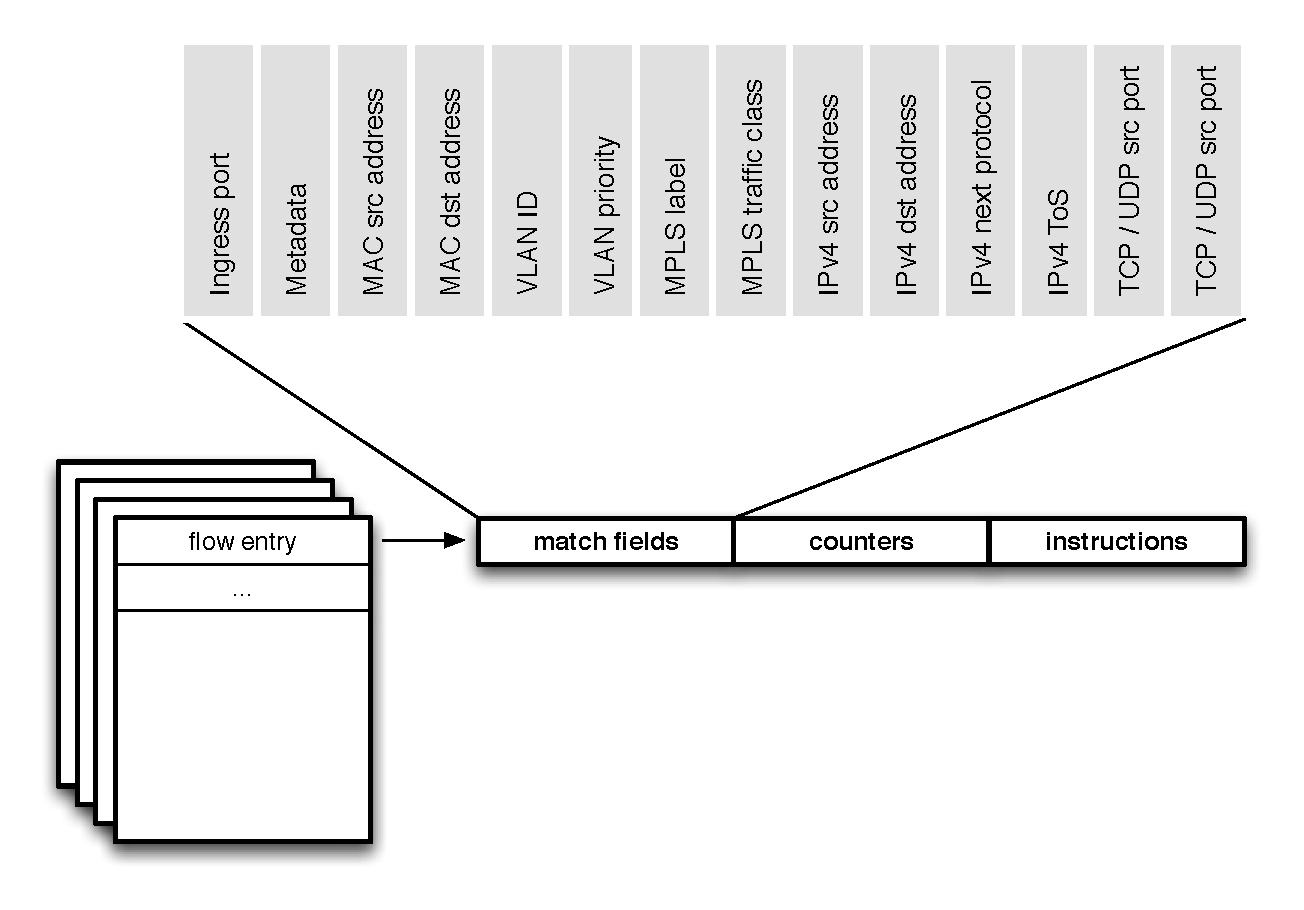
\includegraphics[width=0.9\linewidth]{figures/inflex/ofptable}
    \caption{\label{fig:ofptable}}
    \end{subfigure}
    \caption{Openflow (\subref{fig:ofparch}) architecture and (\subref{fig:ofptable}) flow entry structure.}
\end{figure}

% flow table / entry
An Openflow flow table is composed of multiple flow entries, shown in figure \ref{fig:ofptable}.
Each flow entry is comprised of a pattern to be matched, and the corresponding \emph{instructions} to be executed. 
The \emph{match fields} over which an entry can be compared span from data link to transport layers, covering not only source and destination addresses at each protocol header, but also traffic classes and labels for \ac{VLAN}, \ac{MPLS} and \ac{IPv4} headers.
% instructions?
Additionally, a \emph{counter} keeps track of the number of times the entry is matched.
If more than one matching entry is found, only the entry with the highest \emph{priority} is processed.
Finally, each entry has a pair of associated \emph{timeout} values: a soft timeout, within which an entry is expired if no matching packet arrives, and a hard timeout, by which an entry is irrevocably expired.
If neither timeout is set, a flow entry persists indefinitely.

% processing pipeline
An Openflow switch in turn maintains multiple flow tables.
Every packet received at an Openflow compliant switch is processed along a pipeline which starts by matching the packet against \emph{table 0}.
From this first, default table, corresponding \emph{instructions} may redirect the packet for further matching against another table, thereby chaining processing.
This pipeline processing ceases once a matching entry fails to include a redirection request, with the accumulated instruction set being executed.
In addition to redirections, valid instructions include modifying packet fields, pushing and popping packet tags, and defining through which ports a packet should be forwarded.
%instructions?
If at any point no matching entry is found, the packet is buffered at the switch, and the truncated packet header is sent to the controller.
% controller
Based on the header contents, a controller may decide to install a new flow entry on the switch, or allow the packet to be dropped altogether.
Compared to the underlying, abstracted network elements which compose the data path, the controller is often expected to be entirely software based, and as such is not constrained in how it should process packets.
In practice, this freedom is curbed as increasing complexity at the controller both reduces the rate at which packets are processed, as well as increasing latency for packets buffered at the switch.

% 2 tradeoffs: 
\ac{SDN} provides an abstraction over which different architectural paradigms can be adapted and even coexist.
It does not however prescribe or advocate a specific design -- network practitioners must still consider system properties when grappling with fundamental trade-offs affecting consistency, isolation, reliability and efficiency.
Some of the design considerations for scalable traffic management were previously described in section \ref{section:inflex:design}.
The overall performance of the described architecture is subject to two further critical trade-offs.
% - granularity vs speed
Firstly, the granularity at which flow entries are installed determines how often a controller is called to intervene.
While installing an entry at a flow granularity may allow fine-grained control of resources, it increases both the load on the controller and the latency of the withheld packet.
Conversely, as the granularity becomes coarser, the overhead incurred by the controller is reduced at the cost of flexibility in controlling traffic.
% - omniscience vs fault tolerance
Secondly, controller placement is critical \cite{Heller:2012:CPP:2342441.2342444}.
At one extreme, a fully centralized controller is omniscient within a domain at the expense of reliability and scalability.
At the other, a distributed system of controllers forsakes consistency and liveness in order to scale robustly.

\section{Design considerations}
\label{section:design}

%\subsection{Multipath state}
%\subsection{Network granularity}
%\subsection{Deployment}
%\subsection{Flowlet?}

\ac{SDN} provides an abstraction over which different architectural paradigms can be adapted and even coexist.
It does not however prescribe or advocate a specific design -- network practitioners must still consider system properties when grappling with fundamental tradeoffs affecting consistency, isolation, reliability and efficiency.
This section provides design considerations for scalable traffic management based on observations obtained from the data collected in chapters \ref{chapter:malawi} and \ref{chapter:rate}.

\begin{figure}[t]
    \centering
    \includegraphics[width=4.0in]{figures/inflex/options}
    \caption{\acs{TCP} option usage \label{fig:wscale}}
    \hfill
\end{figure}

Ideally resilience could be implemented at the transport layer alone, for the same motives rate control is best left to end-hosts: ultimately, the host is best positioned to detect end-to-end path faults and can often react over shorter timescales than the network, which must concern itself with reconvergence.
This approach for path fail-over was a significant feature in \ac{SCTP} \cite{rfc4960}.
Unfortunately, deployment of \ac{SCTP} has been negligible in over a decade since standardization, in part because the pervasiveness of middleboxes has significantly affected the ability for new transport protocols to be deployed.
More recently \ac{MPTCP} \cite{Wischik:2008p137} has been proposed addressing many of the same concerns as \ac{SCTP} whilst maintaining the same wire format as \ac{TCP}, thereby ensuring middlebox compatibility.
Despite this, widespread deployment is far from guaranteed, and is largely tied to the rate of \ac{OS} adoption.
As a reference point, figure \ref{fig:wscale} tracks the use of three \ac{TCP} options by overall volume in flows across both directions in the \ac{MAWI} dataset.
While \ac{SACK} is successfully negotiated for most connections, the deployment of the timestamp and windowscale options has lagged.
While the former primarily assists in provide more accurate \ac{RTT} estimates, the latter is critical for performance: without windowscale negotiation, a sender's congestion window cannot exceed 65KB.
Despite offering a clear benefit to both endpoints, being simple to implement and incurring a low overhead, windowscale deployment has only recently picked up momentum, two decades since standardization.
Expecting substantial deployment of a more complex and costly extension such as \ac{MPTCP} over the near future is likely optimistic.
Critically, transport extensions require receiver adoption and are therefore subject to the willingness and ability of users to upgrade their OS.

{\COMMENT missing: PREFLEX problems here. Concept of deployability changed.}

\textbf{Receiver side deployment of even modest \ac{TCP} extensions can be protracted, even when incentives are aligned}. 
Rather than proposing a path for incremental deployment, this work focuses on how to obtain similar benefits immediately -- modifying sender side hosts only. 
A host, however, cannot directly affect routing without changing destination address, which would break legacy \ac{TCP} receiver side implementations. Additional extensions are required on the sender side network to enable multipath forwarding.
Conventional wisdom suggests that maintaining parallel routing planes requires a proportional increase in table size \cite{NingWang:2008p145}, which itself can be subject to exponential growth.
In practice however, this state can be significantly reduced by forsaking coverage for a small proportion of traffic.
Rather than reflect the entirety of its potential path diversity for all traffic, an edge provider can instead provide additional routing planes for only a subset of popular prefixes.

\begin{figure}[t]
    \begin{subfigure}[b]{0.5\linewidth}
        \centering
        \includegraphics[width=3.0in]{figures/inflex/ecdf_network_dst_data_bytes_from_10000.eps}
        \caption{\label{prefix_in}}
    \end{subfigure}
    \begin{subfigure}[b]{0.5\linewidth}
        \centering
        \includegraphics[width=3.0in]{figures/inflex/ecdf_network_dst_data_bytes_to_10000.eps}
        \caption{\label{prefix_out}}
    \end{subfigure}%
    \caption{\acs{CDF} of traffic by announced network prefix for (\subref{prefix_in}) inbound and (\subref{prefix_out}) outbound traffic.\label{fig:prefix}}
    \hfill
\end{figure}

The extent to which such a gain is possible for the \ac{MAWI} dataset is quantified in figure \ref{fig:prefix}, which displays the cumulative distribution function of outbound traffic across network prefixes announced by BGP neighbours.
Over five years, traffic to approximately 340,000 unique prefixes was observed.
Invariably however, an increasing amount is sent to a small group of prefixes -- by 2011, over 50\% of traffic went to the top 100 prefixes alone.
This reflects ongoing structural changes in the Internet architecture as content providers interconnect directly edge, \emph{eyeball} networks, and content becomes increasingly consolidated across a set of large content providers and national and regional ISPs.

\textbf{Multipath routing state can be significantly reduced by covering fewer destinations while still benefiting most traffic}. 
Within the \ac{MAWI} dataset virtually all inbound and outbound traffic could be mapped to 10,000 unique network prefixes. 
Existing \ac{SDN} tools such as RouteFlow \cite{Rothenberg:2012:RRC:2342441.2342445} are already capable of overlaying routing on commodity switches, but the incurred overhead can still be a concern for production networks.
Rather than address the scalability challenges inherent to multipath routing directly, these results suggest that a tangible deployment path lies instead in reducing the scope over which it is applied.


\section{Architecture}
\label{section:inflex:arch}

This section describes INFLEX, an architecture which provides edge domains with greater end-to-end resilience.
Rather than probing paths through active or passive means, the network delegates the responsibility for fault detection to end-hosts.
The system relies on packet marking at the host to select a path through the local domain.
This provides far greater scalability in terms of the proportion of traffic and destinations which can be covered, at the cost of requiring small changes to the end-host \ac{TCP}/\ac{IP} stack.
INFLEX is therefore particularly suited for managed environments, such as datacenters or enterprise networks, which not only have greater control over the end-host operating system, but also generate large volumes of traffic towards destinations which cannot be readily upgraded.

An overview of the proposed architecture as applied to a single domain is shown in figure \ref{fig:inflexarch}.
Hosts are connected to the local network through an Openflow-enabled \emph{edge switch}.
While edge switches typically reside within each physical machine, alternative aggregation levels such as the top of rack or end of row may also be used.
Each switch is configured by a specialized controller which resides locally, referred to as an \emph{inflector}.
The local network is configured by a centralized routing controller to provide multiple \emph{virtual routing planes}.
While these planes are necessarily intradomain in scope, some degree of interdomain diversity can also be achieved by changing egress node.

The core of the architecture relies on repurposing the \ac{DS} field in each \ac{IP} packet to provide an in-band signalling channel between the end-host and the inflector.
The header on inbound traffic is set by the edge switch and read by the host, and is used by the inflector to signal which plane a flow has been assigned to.
The header on outbound traffic is set by the host and read by the edge switch, and is used by the transport protocol to ensure that all traffic for the flow is forwarded along the given plane.
Hosts can request a new plane to be assigned by the inflector in case of an end-to-end path fault; this provides efficient cross-layer failure recovery.
The \ac{DS} standard \cite{Blake:1998p370} reserves a pool of code points for local use identified by setting the right-most bit, henceforth referred to as the INFLEX $flag$.
When set, the rest of the \ac{DS} field should be interpreted as containing two fields, shown in figure \ref{fig:inflexarch}. 
An \ac{INF} $label$, which determines the plane over which a packet is forwarded, and an $echo$ bit, which explicitly signals a request from the host or a reply from the network.
The remainder of the description of INFLEX is split across its main components: the end-hosts, the edge switch and the inflector.

\begin{figure}
    \begin{subfigure}[b]{1.0\linewidth}
    \centering
    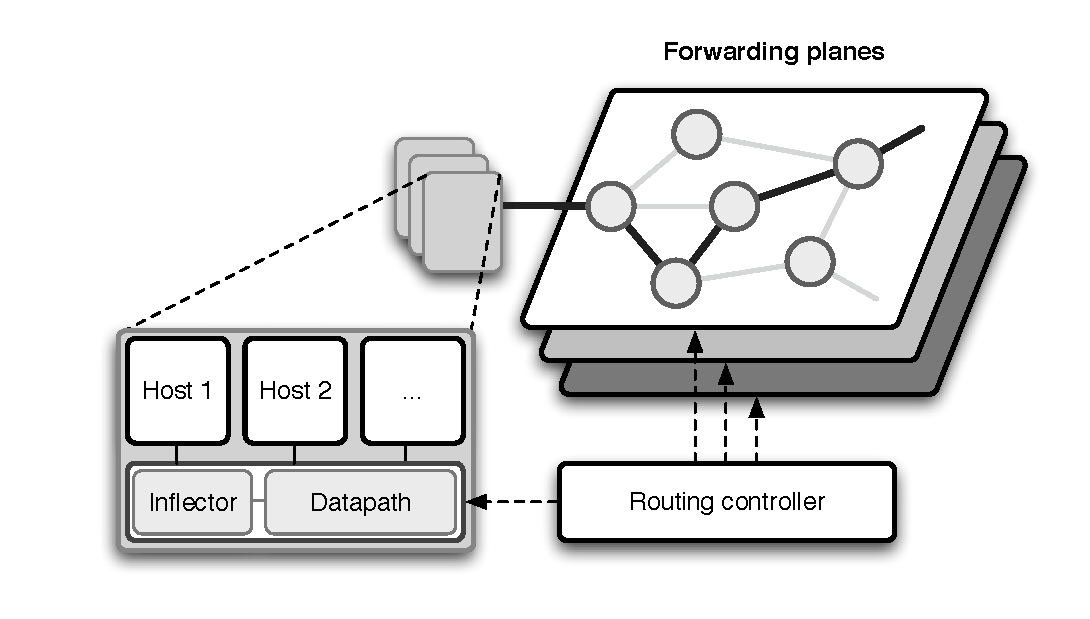
\includegraphics[width=0.7\linewidth]{figures/inflex/arch}
    %\caption{\label{fig:inflexarch}}
    \end{subfigure}
    \begin{subfigure}[b]{1.0\linewidth}
    \centering
    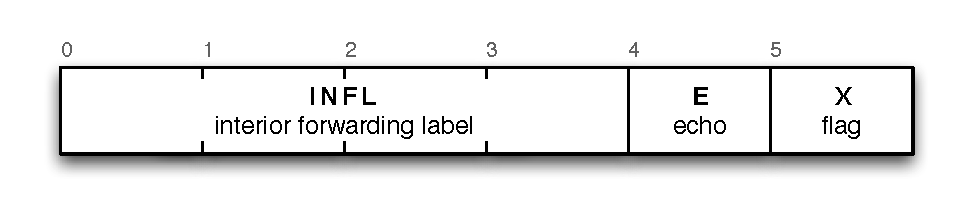
\includegraphics[width=0.5\linewidth]{figures/inflex/header}
    %\caption{\label{fig:inflexheader}}
    \end{subfigure}
    \caption[INFLEX architecture and header.]{INFLEX architecture (above) and header (below). The edge switch forwards traffic across virtual planes set up by a centralized routing service.
    \label{fig:inflexarch}}
\end{figure}

\subsection{INFLEX end-hosts}
\label{section:inflex:host}

INFLEX hosts set the \ac{INF} label of outbound packets according to the value assigned by the inflector, reproducing the path re-feedback design pattern introduced in chapter \ref{chapter:preflex}.
INFLEX however cannot rely on marking by the remote endpoint to trigger network action, as this has been shown to be essentially undeployable.
Instead, path requests are initiated by the sender, which must then await for a network reply piggybacked on a returning packet.

The changes required to support this at the sender side network stack are minimal, and are illustrated in figure \ref{fig:stack}.
Every transport connection occurs over a socket, a local structure containing the variables associated to the ongoing flow.
At the network layer, the local socket has a \ac{DS} value which is copied to every outbound packet (point 1).
Within INFLEX, the transport protocol can trigger a request (point 2), which leads to a network response contained in incoming packets (point 3).

Assume a transport protocol wishes to switch the plane it is currently assigned.
With INFLEX, it can send an \emph{inflection request} by setting the $echo$ bit of the local \ac{DS} field (point 2, figure \ref{fig:stack}).
All subsequent outbound packets will be marked with the resulting value.
The network layer then proceeds to inspect inbound packets, waiting for a network response, as delineated in figure \ref{fig:tcpcode}.
After demuxing an incoming packet, $pkt$, to the corresponding socket, $sock$, a receiver first verifies whether the INFLEX flag is set on the incoming packet (line 2), establishing whether the underlying network supports INFLEX for the given connection.
The receiver must then decide whether it should change the virtual plane the socket is currently assigned.
This can only happen under two conditions.
Firstly, if the \ac{DS} value for the current socket does not have the INFLEX flag set (line 3).
This typically occurs on flow start, where a connection is spawned with a default \ac{DS} value.
Secondly, if the local \ac{DS} value has the echo bit set, there is a \emph{pending} inflection request.
If the incoming packet has the same bit set, it corresponds to the network \emph{reply} (line 4).
Under both previous cases, the connection switches forwarding plane by copy the interior forwarding label from the incoming packet to the local socket, and setting the INFLEX flag (lines 5-6).
These changes are all applied at the \ac{IP} layer -- transport protocols need only to decide when to send inflection requests -- while applications can remain unchanged.

\begin{figure}
    \begin{subfigure}[b]{0.4\linewidth}
        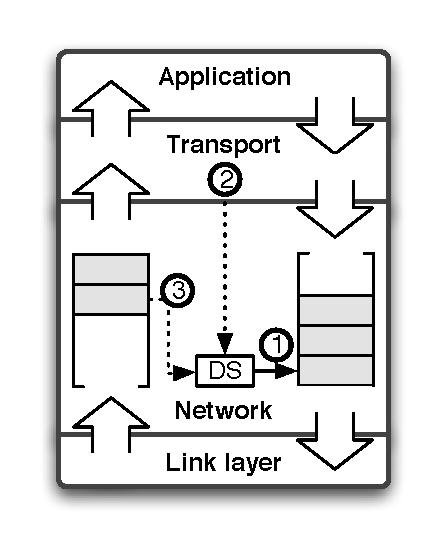
\includegraphics[width=0.9\linewidth]{figures/inflex/stack}
        \caption{\label{fig:stack}}
    \end{subfigure}%
    \begin{subfigure}[b]{0.6\linewidth}
        \vspace*{1.0in}
        \lstset{
        language=C,                % choose the language of the code
        basicstyle=\footnotesize\ttfamily,
        numbers=left,                   % where to put the line-numbers
        stepnumber=1,                   % the step between two line-numbers.
        numbersep=5pt,                  % how far the line-numbers are from the code
        %  backgroundcolor=\color{white},  % choose the background color. You must add \usepackage{color}
        showspaces=false,               % show spaces adding particular underscores
        numberstyle=\scriptsize,
        showstringspaces=false,         % underline spaces within strings
        showtabs=false,                 % show tabs within strings adding particular underscores
        tabsize=2,                      % sets default tabsize to 2 spaces
        captionpos=n,                   % sets the caption-position to bottom
        breaklines=true,                % sets automatic line breaking
        breakatwhitespace=true,         % sets if automatic breaks should only happen at whitespace
        title=\lstname,                 % show the filename of files included with \lstinputlisting;
        }
        \lstinputlisting{\locfolder/tcpapi.c}
        \caption{\label{fig:tcpcode}}
    \end{subfigure}
    \caption[INFLEX host modifications.]{INFLEX (\subref{fig:stack}) host stack and (\subref{fig:tcpcode}) pseudo-code for packet reception.}
\end{figure}

% inflection request
\subsection{The edge switch}

% what is it
The edge switch is primarily responsible for mapping INFLEX marked packets to the appropriate forwarding plane.
On start up its datapath is configured by the local \emph{inflector}, which installs the appropriate flow entries on it in order to construct the processing pipeline in figure \ref{fig:pipeline}.
This pipeline can be partitioned into three distinct blocks, responsible for \emph{triaging}, \emph{policing} and \emph{inflecting} packets.
For clarity, the processing pipeline is conceptually described as a sequence of flow matches across distinct tables.
In practice, an implementer is free to collapse flow tables and entries to improve performance.
An important safeguard is that a legacy pipeline must be present, establishing a default forwarding plane expected to be used by traffic to which INFLEX is not applicable.

\begin{figure}
    \centering
    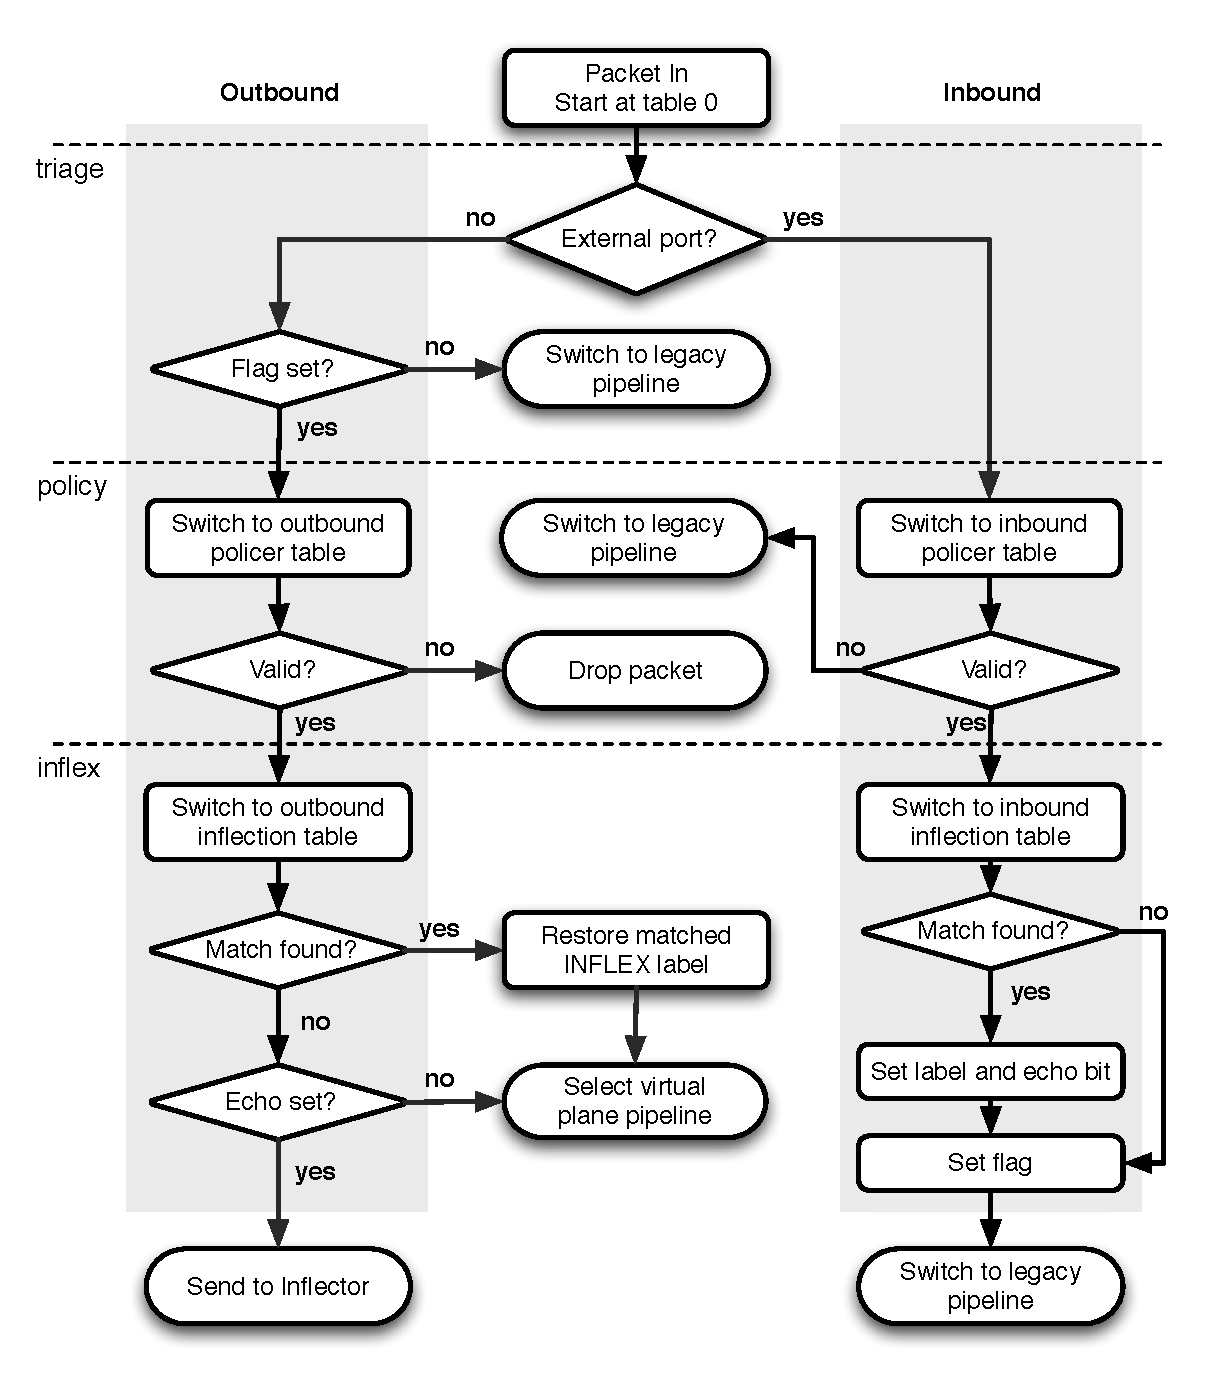
\includegraphics[width=3.5in]{figures/inflex/flowchart}
    \caption{Pipeline installed to the edge switch datapath.}
    \label{fig:pipeline}
\end{figure}

The \emph{triage} phase is responsible for distinguishing whether a packet is \emph{capable} of using INFLEX.
Firstly, INFLEX is only applicable to \ac{IP} packets.
Traffic is then differentiated according to the port on which the packet arrived: if connected to a host, the interface is said to be \emph{internal}, otherwise it is \emph{external}.
Any inbound \ac{IP} traffic may potentially be INFLEX capable and as such can proceed to the next stage.
For outbound \ac{IP} traffic, only packets with the INFLEX flag set require further processing.
Packets for which this flag is not set are assumed to be legacy traffic.

The \emph{policy} phase decides whether a packet is \emph{permitted} to use INFLEX.
For either direction, a packet is compared against a policer table, which contains a set of rules describing local policy concerning INFLEX usage.
The rules applied to each direction however may differ, particularly since outbound packets can be further scrutinized according to the INF $label$.
For example, this allows the outbound policer to enforce which virtual planes are available to specific tenants or applications.
For this reason, the action applied if a packet is matched within the policer table also differs according to direction.
For inbound traffic, a matching rule indicates that the packet does not satisfy local requirements for INFLEX use, and is consequently treated as legacy traffic.
For outbound traffic, a packet is already marked as being INFLEX capable.
Any matching entry therefore indicates that it is in violation of local policy and should consequently be dropped.

Finally, the \emph{inflex} phase processes the respective header and forwards the packet.
A packet is first matched against an \emph{inflection} table in either direction.
This table is detailed in the next section, and can be assumed to contain no matching entry initially.
For outbound traffic, the packet is typically redirected to the  plane mapped by the interior forwarding label.
The one exception are inflection requests, which are forwarded to the local inflector for further processing.
For inbound traffic, the INFLEX flag is marked in order to notify hosts that the flow is INFLEX capable, and the packet is then processed according to the legacy pipeline.

\subsection{The inflector}

% XXX
Each edge switch is controlled by an inflector, an \ac{SDN} controller expected to reside locally.
An inflector is firstly responsible for configuring the underlying datapath according to the previously described pipeline.
Secondly, an inflector must process inflection requests.

Inflection requests require network intervention in assigning a packet to a forwarding plane.
The dynamic nature of this decision process cannot readily be instantiated as a set of static rules at the edge switch, since a same flow must be able to be reassigned to a different plane in case of path faults.
Therefore, inflection requests intercepted at the edge switch must be sent to a controller for further processing.
Rather than overloading a centralized controller however, this decision can be taken locally -- since the inflector manages the local rules associated to each virtual network, it already has full knowledge of the routing table associated to each plane.
Upon receiving such a request, the inflector proceeds in three steps.
It first verifies which virtual networks maintain a valid route for the given destination address.
Given this list of potential planes, it then inspects local policy to verify which planes the packet is allowed to use.
The intercepted packet contains the plane which the flow is currently using -- this plane should be excluded from the candidate list unless there is no other option available.
Finally, a single plane, identified by an interior forwarding label, is selected from the resulting list of candidates.
The selection algorithm is not prescribed by the INFLEX specification, but a reasonable baseline is to select a routing entry proportionally to the assigned route weight.

Having selected an appropriate plane, the inflector installs forwarding rules into either \emph{inflection table}.
In the inbound direction, all packets matching the reverse flow are set to be marked with the corresponding \ac{INF} $label$.
This conveys the selected forwarding plane back to the host.
In the outbound direction, all packets matching the flow are to be processed according to the $label$.
This guarantees that any packet sent between the inflection request and its response are forwarded in a consistent manner.
Rules installed to the inflection tables are ephemeral by nature, with a hard timeout of 1 second (the minimum permitted in the Openflow standard).
This enables per-flow granularity with minimum flow state while also rate limiting inflection requests.
Furthermore, flow entries can be configured to be sent to the controller upon expiry.
This potentially allows the inflector to collect realtime information on the availability of each forwarding plane, allowing for further refinement of the plane selection algorithm.

\section{Performance Analysis}
%4.1) Balancing between two paths with high loss using fixed time unit
% using only loss-based balance in a simple regime where that works.
% Show how this converges quickly when one path suddenly gains
% background traffic (and hence loss).
%4.2) Balance between several paths with high loss and fixed time unit
% in simple regime where that works.
%4.3) Introduce experiment where equi-path is needed for probing and
% conservative is needed for low loss regime.
%4.4) Introduce experiment where time-scale tuning is needed to get
% good assessment of loss in low traffic regime.

We evaluate \ac{PREFLEX} through simulation in ns-3 \cite{ns3}. 
Since \ac{PREFLEX} balances traffic using loss rather than load, there is a need to emulate the end-to-end behaviour of traffic. 
This proves more challenging than analysis of existing traffic engineering proposals which typically only focus on adjusting load, since we wish to verify the impact of \ac{PREFLEX} on end-user metrics. 

\subsection{Methodology}
\label{section:methodology}

For all simulations we will use the topology displayed in figure \ref{fig:topo}. 
The topology links a client domain $C$ to a server domain $S$ through $N$ paths with equal bottlenecks $L_i$, and total bandwidth $B=\sum{L_i}$. 
While a domain is represented as a single entity in figure \ref{fig:topo}, each domain is composed by a traffic generator connected to a router. 
Client $C$ generates $G$ simultaneous \ac{HTTP}-like requests (or ``gets") from $S$ according to a specified distribution, described at the end of this section. 
As traffic flows from $S$ to $C$, the router within $S$ is responsible for balancing traffic over all available paths.

\begin{figure}
    \centering
    \includegraphics[width=2.5in]{figures/cate/topo}
    \caption{Simulation topology}
    \label{fig:topo}
\end{figure}

Across simulations, as the number of paths increases, total bandwidth $B$ and the number of simultaneous requests $G$ is fixed. 
In this manner we wish to analyze how \ac{PREFLEX} balances traffic as the granularity with which it can split traffic becomes coarser.

Since we are interested in evaluating how \ac{PREFLEX} shifts traffic in response to loss, we introduce additional ``dummy" servers $D_i$ which are connected to $C$ through a single path. 
We partition the total simulation time $T$ into $N+2$ intervals starting on $s_i$, in which $s_0$ and $s_{N+1}$ have no traffic to $D_i$. 
Starting at time $s_i$, client $C$ generates $g_i$ requests to $D_i$ according to the same distribution as used to server $S$. 
All requests to $D_i$ end at time $s_{N+1}$. 
Equation \eqref{eq:si} sets the start time $s_i$ for requests to $D_i$ as a function of total simulation time $T$ and number of paths $N$. 
Likewise, equation \eqref{eq:gi} sets the number of simultaneous requests $g_i$ to $D_i$ as a function of $G$, the total number of requests to $S$, and $N$.
\begin{equation}
s_i = T\frac{i}{N+2}
\label{eq:si}
\end{equation}
\begin{equation}
\theta_i = \frac{\frac{1}{N+1-i}}{\sum{\frac{1}{N+1-i}}},  g_i = G\theta_i.
\label{eq:gi}
\end{equation}

Figure \ref{fig:demand} illustrates the number of simultaneous gets from $C$ to $D_i$ for $N=2$ (used in the example shown in figure \ref{fig:two}) and $N=4$. 
Generating cross-traffic in this manner serves two purposes. 
Firstly, $\sum{g_i}=G$, so independently of the number of concurrent paths, the maximum load in the system is $2G$. 
However, as the number of paths increases, the fluctuation in load for each path becomes smaller, and so we will stress the sensitivity with which \ac{PREFLEX} balances traffic. 
Secondly, the number of requests for each $D_i$ over time is the same. 
Over timescale $T$, equalisation appears to be an acceptable strategy, however within each interval we will show it performs poorly achieve consistent behaviour. 
This is a fundamental limitation of offline traffic engineering, which is calculated over very long timescales and is unable to adapt as traffic routinely shifts.


\begin{figure}
    \begin{subfigure}[b]{.5\linewidth}
        \centering
        \includegraphics[width=2.25in]{figures/cate/dummy2-crop.pdf}
        \caption{$N=2$}\label{fig:1a}
    \end{subfigure}%
    \begin{subfigure}[b]{.5\linewidth}
        \centering
        \includegraphics[width=2.25in]{figures/cate/dummy4-crop.pdf}
        \caption{$N=4$}\label{fig:1b}
    \end{subfigure}
    \caption{Number of requests from $C$ to cross traffic servers $D_i$ for different values of $N$}
    \label{fig:demand}
\end{figure}

We now specify the settings common to all simulations, including those previously shown in figure \ref{fig:two}. 
Total simulation time $T$ is set to $1200$ seconds, while total bandwidth $B$ is fixed at $240$Mbps. 
The number of requests $G$ sent from $C$ to $S$ is set to 240. 
Upon completing, a request is respawned after an idle period following an exponential distribution with a $15$s mean. 
Transfer size follows a Weibull distribution with an average value of $2$MB. 
These values attempt to reflect traffic to a single prefix with a file size that mimics the small but bursty nature of web traffic, which does not lend itself to being balanced by the end-host. 
\ac{PREFLEX} is configured with $\beta_E = 0.05$, $\mu_{min}=0.01/N$ and $\delta=0.005$.

\subsection{Varying bottleneck distribution}

We start by examining the case where all bottlenecks share the same bandwidth, $L_i=B/N$, and compare \ac{PREFLEX} to equalisation, which mimics traffic engineering techniques based on hashing flow tuples and assigning them to a path. 
The goodput, calculated as the total data transfered to client $C$ by flows completed within $T$, is shown for both equalisation and \ac{PREFLEX} methods in figure \ref{fig:goodputeq}. 
While both saturate most available bandwidth, equalisation leads to disproportionate distribution of goodput amongst competing traffic. 
As loss is not equalised over all paths, the amount of goodput achieved by servers $D_i$ differs despite demand being similar.

Equalisation, even when weighted according to local link capacity, is often prone to remote bottlenecks. 
We investigate the effect of differing bottlenecks by repeating previous simulations with the same total bandwidth $B$, but with $L_i$ set proportionally to $B$ in a similar manner to \eqref{eq:gi}, that is $L_i = \theta_i B$.


\begin{figure}
    \centering
    \includegraphics[width=4in]{figures/cate/eqbw}
    \caption{Goodput relative to $B$ achieved by each server for equal capacity links.}
    \label{fig:goodputeq}
\end{figure}

Figure \ref{fig:goodputeq} shows the goodput as a proportion of total link bandwidth for the case where all links have equal bandwidth. 
We vary the number of links $N$, and for each case compare equalisation (as illustrated in \ref{fig:twoequal}) and \ac{PREFLEX} as the balancing methods used. 
The bulk of goodput originates from server $S$, which is the only domain to be connected to all links.  
If traffic is correctly balanced, we expect to see servers $D_{1-N}$ generate the same amount of goodput.

In this scenario, equalisation can be seen as the optimal static TE solution, yet both approaches bear similar performance. 
With no knowledge of topology, link bandwidth or expected traffic matrices, \ac{PREFLEX} is able to adequately mimic the performance of the static TE solution for the case where such an approach is best suited.


\begin{figure}
    \centering
    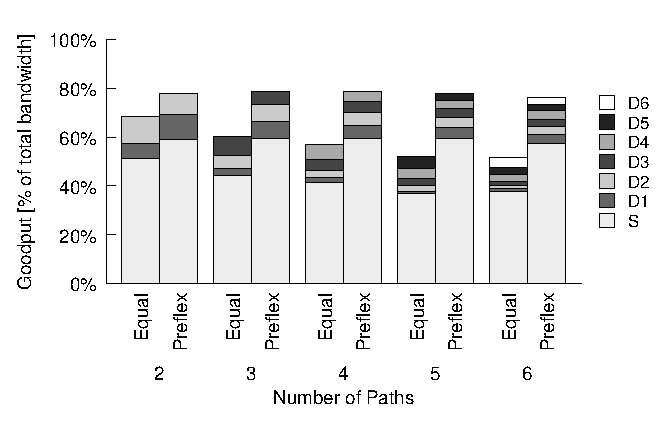
\includegraphics[width=4in]{figures/cate/diffbw}
    \caption{Goodput relative to $B$ achieved by each server for different capacity links.}
    \label{fig:goodputdiff}
\end{figure}

Where bottleneck bandwidth is unequal however equalisation proves inadequate. 
Once again comparing goodput (figure \ref{fig:goodputdiff}) we highlight two significant shortcomings of equalisation which \ac{PREFLEX} overcomes. 
Firstly, goodput for $S$ drops as $N$ increases. 
Unable to realize it is overloading a path, equalisation is reduced to sending traffic over each link at approximately the same rate as the most congested link. 
In contrast, \ac{PREFLEX} detects congestion and adapts accordingly. 
Secondly, the incorrect distribution of traffic due to equalisation in $S$ distorts the goodput of others servers. 
While in \ac{PREFLEX} goodput from $D_{1-N}$ is perfectly balanced, with equalisation traffic crossing the most congested links are directly affected by another domain's inability to distribute its traffic appropriately.
It may seem unfair to judge equalisation for cases where there is a mismatch in link capacity, however this mismatch between link weight and path capacity arises regularly as operators continue to adjust traffic engineering according to local conditions, with little thought spared for the impact this may have further downstream.

\begin{figure}
    \centering
    \includegraphics[width=3.2in]{figures/cate/duration}
    \caption{Mean average flow completion time for equal and differing bottleneck links.}
    \label{fig:duration}
\end{figure}

This impact is in turn perceived by users, who experience longer flow completion times, as shown in figure \ref{fig:duration}. 
In the equal bandwidth case the flow completion time is similar for both balancers.  
Where bandwidth differs however, \ac{PREFLEX} outperforms equalisation and maintains a stable performance when balancing over all six paths.  
This shows that the algorithm scales well as the number of available paths increases. 


\chapter{Conclusions}
\label{chapter:conclusions}

The presented body of work identifies opportunities and explores strategies for resource pooling through the application of \emph{re-feedback}.
This chapter summarises these findings in light of the original problem statement:

\begin{quote}
\textit{
Given the nature of Internet traffic, how can the current architecture be realigned to facilitate resource pooling at both network and transport layers?
}
\end{quote}

\renewcommand{\descriptionlabel}[1]{\hspace{\labelsep}\textbf{#1}}
\begin{description}
\item[Efficient]
%cate
\LOREM
\item[Flexible]
%TE, opt-out
\LOREM
\item[Robust]
%inflex
\LOREM
\end{description}

%tip
Resource pooling has evolved to being performed by different stakeholders unilaterally.
End-hosts, network operators and content providers all attempt to pool traffic by differing means, and in a potentially conflicting manner.
While recent work has lent credence to pushing resource pooling towards the edge, this ignores the tussle over how traffic is managed between these stakeholders.
Path diversity is in the network, and operators attempt to exploit it through a combination of route optimization and traffic balancing.
Collectively, these traffic engineering methods assist networks in minimizing the costs incurred by shifting traffic.
Conversely, hosts are increasingly capable of pooling traffic across paths either through the use of overlay networks or multipath congestion control, neither of which necessarily share the objectives of the underlying network.
The problem statement arises from the confluence of these two trends: given the nature of Internet traffic, how can the current architecture be realigned to facilitate resource pooling at both network and transport layers?

\section{Summary of contributions}

The core of the proposed thesis revolves around Internet architecture and as such is of most immediate interest to protocol designers.
The many contributions presented however carry much wider appeal, and can be classified under 

%Network operators, application developers and ?

\subsection{Internet traffic characterisation}

% lit review
This thesis began by providing a broader context within which to frame the evolution of resource pooling.
Chapter \ref{chapter:resourcepooling} traces how successive waves of new stakeholders and novel applications have influenced and shaped the protocols and tools which form the Internet.
Importantly, this chapter highlights traffic management as an architectural afterthought and identifies a pertinent problem:
, with end-hosts, network operators and content providers alike pooling traffic unilaterally through differing means.


% malawi intro
As with any distributed system however, the Internet remains in a constant state of flux.
\LOREM
Chapter \ref{chapter:malawi} provides a significant reappraisal of past work in characterizing Internet traffic
% the flattening, delay 

% rate limitations
The main contribution in this study however was a re-evaluation of commonly held assumptions regarding Internet flow rates by systematically identifying artificial constraints to \ac{TCP} traffic throughput across three categories: \emph{application pacing}, \emph{host limiting} and \emph{receiver shaping}. 
The resulting analysis shows that flow rates are not typically dictated by \ac{TCP} congestion control alone, and has significant implications on how to reason about resource sharing in particular.
The findings equally confirm that \ac{TCP} throughput is mostly determined by the actions of the sender and that continuing \acf{OS} updates have progressively lifted many of the limitations inherent to socket buffer sizes. 
These changes have allowed smaller flows to increase throughput at a far higher rate than larger flows, which are more often than not affected by other mechanisms of traffic shaping.
This means that, although there is a correlation between flow volume in bytes and throughput, the relationship between the two is non-linear and has changed with time.

% implications for resource pooling
These changes were perhaps foreseeable given the all-encompassing nature of the \ac{IP}: the Internet will continue to assimilate the characteristics of the networks it progressively replaces.


% the evolution of existing Internet architecture is less clear.


% tip
%The Internet is in a constant state of flux, as remarkable in its ability to seamlessly accomodate new stakeholders as it is in reinventing itself to meet new requirements. 
%This disruptive nature often hinders our ability to discern between the evolution of the Internet and the ebb and flow of otherwise highly localized events. Under these circumstances, 
%the usefulness of longitudinal studies is twofold: they both offer a perspective on the underlying long term behaviour of a system as a whole, and provide a context under which transient events can be better understood.



Having reconstructed individual flows, the results are aggregated using an external routing information dataset and relate how each aritificial constraint arises in different contexts and affects different stakeholders over time. 
In particular, we show that host limitations have largely been lifted for small flows, with the windowscale option increasing threefold to cover over 80\% of all inbound traffic by the end of 2011. 
Understanding the characteristics of Internet traffic is intrinsic to designing any form of resource pooling.
For long-lived flows, the transport layer has sufficient time to collect information on network state to efficiently pool traffic across multiple paths.
If traffic is dispersed across many prefixes, scaling dynamic traffic engineering may be problematic.
By relating five years of packet traces from an interdomain transit link with topological and geographic information, preliminary results suggest neither is strictly true.
The continuing consolidation of traffic for both inbound and outbound directions allows most traffic to be balanced by manipulating a small number of traffic prefixes.
This work has corroborated previous findings \cite{Labovitz:2010p175} showing a shift in content distribution, with \acf{P2P} applications being slowly replaced by \acfp{CDN} and \acf{OCH} infrastructure.
The novelty has come from being able to relate traffic trends at a finer granularity, both by reconstructing \ac{TCP} behaviour and relating these changes to network prefixes, which can in turn be used to assess the practicality of dynamic traffic engineering methods.


\subsection{Architectural realignment}

% relation to state of art
This thesis set off by exploring the use of re-feedback, originally proposed by Briscoe et al. \cite{}, for purposes other than accountability.
%While the expectation that networks could be held accountable for congestion conferred interesting properties
Removing the expectation that networks would be held accountable for congestion lead to a fundamentally poorer architecture, but one in which enforcement

%is purpose resulted in a significantly

To this end, \ac{LEX} was proposed in \ref{chapter:preflex} as a simplified mechanism for echoing loss back into the network.

The point of departure of this thesis was provided by 
starting point of this 
Loss exposure was since pursued independently by the \ac{CONEX} working group.

% pref
Arguably the single most valuable legacy of this work was in proposing \acf{PREF} as a cross-layer signalling mechanism between the transport and network layer, first presented in chapter \ref{chapter:preflex}.
Within the self-imposed constraints of \ac{IPv4} deployability, the resulting mechanism is necessarily simple, but also shown to be surprisingly versatile, enabling novel end-to-end traffic management techniques such as congestion balancing, presented in chapter \ref{chapter:cate}, and resilient path fail-over, presented in chapter \ref{chapter:inflex}.
Historically, the \ac{PREF} field can be interpreted as a synthesis of the previously sanctioned uses for the same header space: neither strictly abiding by the thesis that end-hosts should independently determine their own \acf{ToS}, nor aligning itself with the antithetical view that the network alone should establish \acf{DS}.
In many respects, it is a stronger ideological heir to the original design philosophy of the \ac{DARPA} internet protocols. 
In deliberating on the success of the latter in \cite{Clark:1988p478}, Clark concludes by identifying shortcomings of the datagram model given requirements which had not originally been contemplated:

While

% lex

% inflex





% tip
Given the Internet architecture should not dictate the outcome of the tussle between end-host and network solutions for resource pooling, the \ac{PREFLEX} architecture attempts to make both aware of each other.
\acf{LEX} transmits information on loss as viewed by the transport layer to network resources, allowing traffic engineering to be performed taking into account end-to-end path quality.
\acf{PREF} offers the ability for the network to select and offer paths to hosts, thereby unlocking the path diversity which already exists at stub domains such as \acp{ISP}, \acp{CDN} and enterprise networks.

\ac{PREFLEX} permits more efficient, reliable and flexible traffic balancing whilst allowing for a range of outcomes in how burden of resource pooling is shared between host and network.
One extreme outcome, in which the network is responsible for all resource pooling, is explored in depth in chapter \ref{chapter:cate}.
A congestion balancer is derived in which \ac{PREFLEX} can reap much of the benefit of \ac{MPTCP} by balancing flowlets according to loss.
Unlike most existing \ac{TE} methods, \ac{PREFLEX} is designed to minimize the impact of route changes on the transport layer and as such is assessed by its impact on transport metrics rather than traffic aggregates.
The use of congestion balancing in the network not only leads to a more efficient use of network capacity, but also a reduction of flow completion times for flows.

    \textbf{Evolution of flowlets}. Recent work on video streaming \cite{Rao:2011p547} , which represents a significant portion of Internet traffic, 
    has shown different sending strategies are adopted depending on the application type (web browser or native) and container (HTML5 or Flash).
    The most popular strategies rely on on/off sending patterns of varying chunk sizes, a form of rate-limiting may affect how efficiently \ac{TCP} can probe for bandwidth.
    A methodology for processing flowlets within the \ac{MAWI} packet traces is being developed to understand the evolution of flowlet sizes within Internet traffic and quantify the potential benefits of balancing at a flowlet granularity as proposed in \ac{PREFLEX}.

{\COMMENT
    %copy pasted from INFOCOM intro
% INFLEX
This paper presents INFLEX, an \ac{SDN}-based architecture for cross-layer network resilience which provides on-demand path fail-over for \ac{IP} traffic. 
The architecture is both unilaterally deployable, providing benefits even when adopted by individual domains, and inherently end-to-end, potentially covering third party failures.
INFLEX operates by allowing an \ac{SDN}-enabled routing layer to expose multiple \emph{routing planes} to the transport layer. 
Hence, traffic can be shifted by one routing plane to another as a response to end-to-end failure detection.
Since INFLEX operates as an extension to the network abstraction provided by \ac{IP}, it can be used by all transport protocols.
At the host, the proposed architecture allows transport protocols to switch network paths at a timescale which avoids flow disruption and which can be transparently integrated into existing congestion control mechanisms.
Within the network, INFLEX provides both greater insight into end-to-end path quality, assisting fault detection, and more control over flow path assignment, enabling more effective fault recovery. 
In addition to describing our architecture design and justifying our design choices with extensive network measurements, we also implement INFLEX and verify its operation experimentally. 
We make our modifications to both the \ac{TCP}/\ac{IP} network stack and a popular Openflow controller \cite{pox} publicly available.
}

\subsection{Facilitating resource pooling}

The core objective of the proposed architectural changes was to \emph{facilitate} resource pooling at both network and transport layers.
To this end, auxiliary mechanisms were proposed to demonstrate the practicality of applying re-feedback principles for traffic management purposes.

% congestion balancing
Chapter \ref{chapter:cate} presented a congestion balancer.
\LOREM
\LOREM

% inflex resilience
Chapter \ref{chapter:inflex} 

Both contributions purposely addressed existing concerns which are currently solved in a convoluted manner.


%tip
The current architecture imposes constraints on how resource pooling can be performed.

\section{Future work}


The task of processing multiple data sources to produce \ac{MALAWI} was a significant undertaking which has only recently started to bear results.
Chapter \ref{chapter:malawi} presents the preliminary results of relating the spatial, behavioural and longitudinal properties of Internet transit traffic.
Moving forward, future work on \ac{MALAWI} will focus on investigating properties of traffic which are relevant to \ac{PREFLEX}:

\begin{itemize}
\item{
    \textbf{Delay}: The effect of path latency has not been considered in designing \ac{PREFLEX}.
    In balancing by congestion delay is implicitly taken into account when using a conservative approach, as \ac{TCP} presents a bias towards shorter \acp{RTT}.
    In some cases however the difference in delay between paths may be significant enough to affect overall performance.
    In its current guise \ac{PREFLEX} does not discard the usage of paths, even if they present a impractically large end-to-end delay.
    The simplest way to avoid their usage would be to render paths unusable through the routing architecture, but this cannot be done in an automated manner taking into account delay.
    Work is undergoing in quantifying the differences in delay between paths to a same destination for the \ac{MAWI} dataset, and the repercussions that may have on \ac{PREFLEX}.
}
\end{itemize}

Furthermore, since the inception of \ac{PREFLEX}, work within \ac{MALAWI} and concurrent research has justified many of its design choices, but also put into question some of its traits.
In moving forward the following issues must be addressed:

\begin{itemize}
\item{
    \textbf{Loss}: The \ac{MAWI} traces demonstrate that outbound loss is receding.
    Whether this is due to higher bandwidth, changes in application usage or shift in where traffic flows to is inconsequent: for many network prefixes, the resolution of loss as a signal may be too low to be used effectively by \ac{PREFLEX}.
    In part, this is due to the scaling properties of \ac{TCP} which dictate loss events will be increasingly spaced out in time as bandwidth increases.
    \ac{PREFLEX} would function best with less conservative forms of congestion control, such as Relentless \ac{TCP} or \ac{DCTCP}.
    In the absence of such approaches, it is important to identify under what conditions congestion balancing makes sense, and improve the design of \ac{PREFLEX} accordingly.
}

\item{
    \textbf{Pricing}: Congestion balancing represents a corner case where network and hosts are fully aligned. 
    Much of the motivation for this work derived from the discrepancy how network resources are shared and how they are priced.
    Whether applied to \acp{ISP} or data centers, an operator should be able to influence how traffic is routed in order to minimize costs.
    This requires extending the work in section \ref{chapter:cate} to cover popular pricing models such as the 95th percentile.
}
\end{itemize}

Results from \ac{MALAWI} corroborate the increase in proportion of traffic originating in co-location sites already described in \cite{Labovitz:2010p175}.
Data centers provide an ideal setting for \ac{PREFLEX} as a single entity is responsible for managing infrastructure, alleviating the possibility of hosts overriding network preferences.
The simplicity of the sender-side changes mean \ac{PREFLEX} can be implemented in the hypervisor and run transparently to hosted virtual machines, an approach already used in \cite{Wu:2010p556}.
In comparison to the use of \ac{MPTCP} in data center traffic \cite{Raiciu:2011p539}, \ac{PREFLEX} may be more suitable for \acp{CDN} dominated by short flows such as web traffic, rate-limited flows such as video streaming, or traffic bound for legacy hosts which cannot support changes to the networking stack.

\COMMENT{Generality of TCP: initial assertion was that TCP was too general.. must infer everything from the network for each flow. Final conclusion is that ultimately this conservativeness is justified and useful, since lack of assumptions makes it adaptable in ways we still can't foresee.
Measurement also likely an inflection point in time, where need for new transport requirements collapse on TCP / UDP. The pluralism which first manifested itself as multiple congestion control algorithms moves onto multiple transport paradigms.}


\section{Closing remarks}


\begin{quote}
%\textit{It proved more difficult than first hoped to provide multiple types of service without explicit support from the underlying networks. The most serious problem was that networks designed with one particular type of service in mind were not flexible enough to support other services.}

%\textit{While the datagram has served very well in solving the most important goals of the Internet, it has not served so well when we attempt to address some of the goals which were further down the priority list.  For example, the goals of resource management and accountability have proved difficult to achieve in the context of datagrams.  As the previous section discussed, most datagrams are a part of some sequence of packets from source to destination, rather than isolated units at the application level.  However, the gateway cannot directly see the existence of this sequence, because it is forced to deal with each packet in isolation.  Therefore, resource management decisions or accounting must be done on each packet separately.  Imposing the datagram model on the internet layer has deprived that layer of an important source of information which it could use in achieving these goals.}

\textit{
While the datagram has served very well in solving the most important goals of the Internet, it has not served so well when we attempt to address some of the goals which were further down the priority list.  
For example, the goals of resource management and accountability have proved difficult to achieve in the context of datagrams.  
(...)
It would be necessary for the gateways to have flow state in order to remember the nature of the flows which are passing through them, but the state information would not be critical in maintaining the desired type of service associated with the flow. Instead, that type of service would be enforced by the end points, which would periodically send messages to ensure that the proper type of service was being associated with the flow.
(...)
I call this concept ``soft state,'' and it may very well permit us to achieve our primary goals of survivability and flexibility, while at the same time doing a better job of dealing with the issue of resource management and accountability.
}
\end{quote}




\bibliographystyle{IEEEtran}
{\footnotesize \bibliography{noms}}

\end{document}
